% ============================================================
%  Příprava na maturitu – Elektrotechnika
%  SOUHRNNÝ TAHÁK A KLÍČOVÉ SOUVISLOSTI
% ============================================================

\documentclass[a4paper,10pt]{article}

\usepackage[T1]{fontenc}
\usepackage[utf8]{inputenc}
\usepackage[left=2.0cm, right=1.8cm, top=1.8cm, bottom=1.8cm]{geometry}
\usepackage{parskip}
\usepackage{xcolor}
\usepackage{tabularx}
\usepackage{booktabs}
\usepackage{tikz}
\usepackage{mdframed}
\usepackage{amsmath}
\usepackage{circuitikz}

\usetikzlibrary{arrows.meta, positioning, shapes.geometric, calc}

% --- Barvy ---
\definecolor{accent}{HTML}{1A3A5C}
\definecolor{lightblue}{HTML}{EAF2F8}
\definecolor{lightyellow}{HTML}{FDFBE4}
\definecolor{lightgreen}{HTML}{EAF7EA}
\definecolor{lightred}{HTML}{FDE8E8}

% --- Boxy ---
\newmdenv[backgroundcolor=lightblue,linecolor=accent!40,roundcorner=4pt,innertopmargin=6pt,innerbottommargin=6pt,innerleftmargin=8pt,innerrightmargin=8pt]{pojmybox}
\newmdenv[backgroundcolor=lightyellow,linecolor=accent!30,roundcorner=4pt,innertopmargin=6pt,innerbottommargin=6pt,innerleftmargin=8pt,innerrightmargin=8pt]{vysvetlenibox}
\newmdenv[backgroundcolor=lightgreen,linecolor=accent!40,roundcorner=4pt,innertopmargin=6pt,innerbottommargin=6pt,innerleftmargin=8pt,innerrightmargin=8pt]{vzorcebox}

\begin{document}

\section*{\centering \huge Elektrotechnika: Velký maturitní souhrn}

\begin{pojmybox}
\centering \textbf{Základní pilíře:} Vše v elektrotechnice vychází z rovnováhy mezi zdrojem, polem a spotřebičem.
\end{pojmybox}

% ================================================================
\subsection*{1. Evoluce Ohmova zákona – Vše souvisí se vším}

Ohmův zákon není jen $U=R \cdot I$. Jeho princip (Napětí = Odpor $\times$ Proud) prostupuje každým okruhem v jiné formě:

\begin{center}
\begin{tabularx}{\linewidth}{l X l}
\toprule
\textbf{Oblast} & \textbf{Forma Ohmova zákona} & \textbf{Klíčová veličina} \\
\midrule
\textbf{Stejnosměrný proud} & $U = R \cdot I$ & $R$ (Rezistance) \\
\textbf{Střídavý proud} & $U = Z \cdot I$ & $Z$ (Impedance) \\
\textbf{Magnetické obvody} & $U_m = R_m \cdot \Phi$ & $R_m$ (Mag. odpor) \\
\textbf{Elektrostatika} & $U = \int E \cdot dl$ & $E$ (Intenzita) \\
\textbf{Polovodiče} & $U = U_F + r_d \cdot I$ & $r_d$ (Diferenciální odpor) \\
\bottomrule
\end{tabularx}
\end{center}

\begin{center}
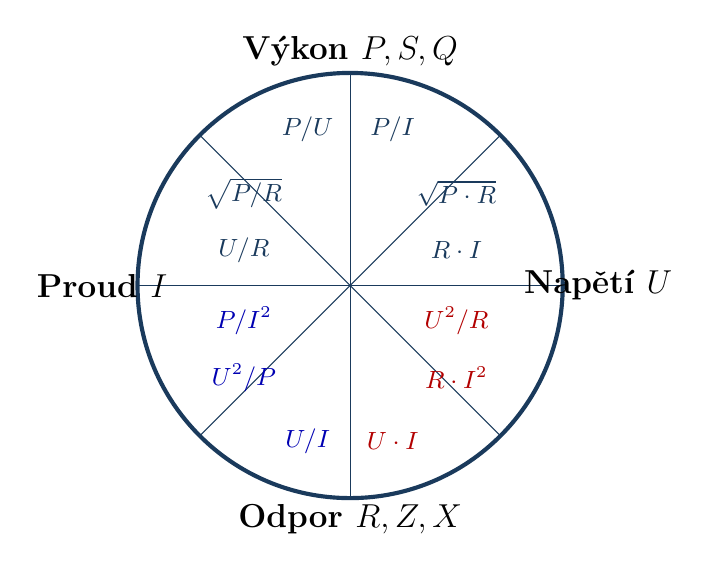
\begin{tikzpicture}[scale=0.9, every node/.style={font=\small}]
    % Ohmův kruh
    \draw[line width=1.5pt, accent] (0,0) circle (3cm);
    \draw[accent] (-3,0) -- (3,0);
    \draw[accent] (0,-3) -- (0,3);
    \draw[accent] (2.12, 2.12) -- (-2.12, -2.12);
    \draw[accent] (-2.12, 2.12) -- (2.12, -2.12);

    \node at (0, 3.3) {\large \textbf{Výkon $P, S, Q$}};
    \node at (3.5, 0) {\large \textbf{Napětí $U$}};
    \node at (0, -3.3) {\large \textbf{Odpor $R, Z, X$}};
    \node at (-3.5, 0) {\large \textbf{Proud $I$}};

    % Výpočty napětí
    \node[accent] at (1.5, 0.5) {$R \cdot I$};
    \node[accent] at (1.5, 1.3) {$\sqrt{P \cdot R}$};
    \node[accent] at (0.6, 2.2) {$P / I$};

    % Výpočty proudu
    \node[accent] at (-1.5, 0.5) {$U / R$};
    \node[accent] at (-1.5, 1.3) {$\sqrt{P / R}$};
    \node[accent] at (-0.6, 2.2) {$P / U$};

    % Výpočty výkonu
    \node[red!70!black] at (0.6, -2.2) {$U \cdot I$};
    \node[red!70!black] at (1.5, -1.3) {$R \cdot I^2$};
    \node[red!70!black] at (1.5, -0.5) {$U^2 / R$};

    % Výpočty odporu
    \node[blue!70!black] at (-0.6, -2.2) {$U / I$};
    \node[blue!70!black] at (-1.5, -1.3) {$U^2 / P$};
    \node[blue!70!black] at (-1.5, -0.5) {$P / I^2$};
\end{tikzpicture}
\end{center}

% ================================================================
\subsection*{2. Srovnání polí – Statika vs. Dynamika}

\begin{vzorcebox}
\begin{tabularx}{\linewidth}{X X}
\textbf{Elektrostatické pole ($Q$)} & \textbf{Magnetické pole ($I$)} \\
\midrule
Intenzita: $E = F/Q = U/d$ [V/m] & Indukce: $B = \Phi/S$ [T] \\
Kapacita: $C = Q/U$ [F] & Indukčnost: $L = \Phi/I$ [H] \\
Energie: $W_e = \frac{1}{2} C U^2$ & Energie: $W_m = \frac{1}{2} L I^2$ \\
Konstanta: $\varepsilon = \varepsilon_0 \varepsilon_r$ & Konstanta: $\mu = \mu_0 \mu_r$ \\
\end{tabularx}
\end{vzorcebox}

% ================================================================
\subsection*{3. Reakce prvků v AC obvodu (Fázory)}

Pamatuj si pravidlo: \textbf{„Na cívce se napětí předbíhá, na kondenzátoru se Napětí opožďuje.“}

\begin{center}
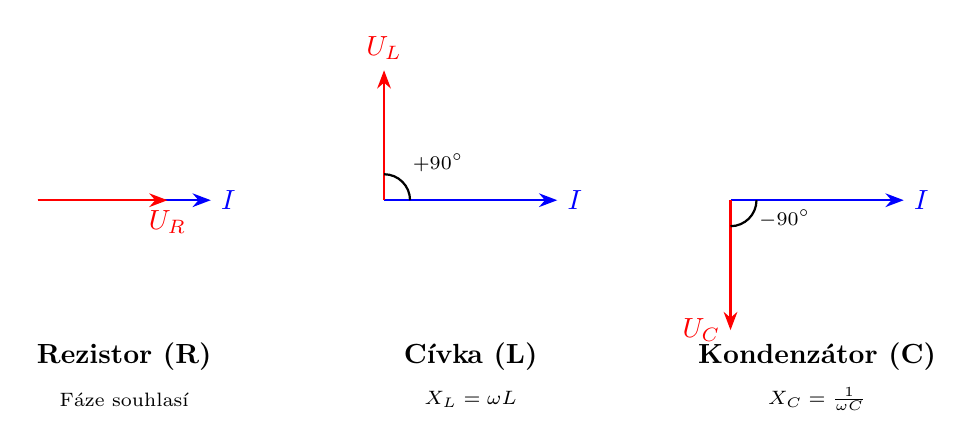
\begin{tikzpicture}[>=Stealth, thick, scale=1.1]
    % Rezistor
    \begin{scope}[xshift=0cm]
        \draw[->, blue] (0,0) -- (2,0) node[right] {$I$};
        \draw[->, red] (0,0) -- (1.5,0) node[below] {$U_R$};
        \node at (1, -1.8) {\textbf{Rezistor (R)}};
        \node[font=\scriptsize] at (1, -2.3) {Fáze souhlasí};
    \end{scope}
    % Cívka
    \begin{scope}[xshift=4cm]
        \draw[->, blue] (0,0) -- (2,0) node[right] {$I$};
        \draw[->, red] (0,0) -- (0,1.5) node[above] {$U_L$};
        \draw (0.3,0) arc (0:90:0.3) node[midway, above right, font=\scriptsize] {$+90^\circ$};
        \node at (1, -1.8) {\textbf{Cívka (L)}};
        \node[font=\scriptsize] at (1, -2.3) {$X_L = \omega L$};
    \end{scope}
    % Kondenzátor
    \begin{scope}[xshift=8cm]
        \draw[->, blue] (0,0) -- (2,0) node[right] {$I$};
        \draw[->, red] (0,0) -- (0,-1.5) node[left] {$U_C$}; % Popisek posunut vlevo
        \draw (0.3,0) arc (0:-90:0.3) node[midway, right, font=\scriptsize] {$-90^\circ$};
        \node at (1, -1.8) {\textbf{Kondenzátor (C)}};
        \node[font=\scriptsize] at (1, -2.3) {$X_C = \frac{1}{\omega C}$};
    \end{scope}
\end{tikzpicture}
\end{center}

% ================================================================
\subsection*{4. Topologie sítí a Bezpečnost (Klíčová čísla)}

\begin{vysvetlenibox}
\begin{itemize}
    \item \textbf{230 V / 400 V:} Fázové vs. Sdružené napětí ($U_s = \sqrt{3} \cdot U_f$).
    \item \textbf{TN-S:} Síť, kde PE a N jsou vedeny odděleně (5 drátů).
    \item \textbf{30 mA:} Mezní reziduální proud chrániče pro ochranu osob.
    \item \textbf{50 V:} Bezpečné střídavé napětí v normálním prostředí.
    \item \textbf{IP20 vs IP44:} Základní krytí vs. krytí do vlhka (koupelny).
\end{itemize}
\end{vysvetlenibox}

% ================================================================
\subsection*{5. Jak "přemýšlet" u strojů (Rychlý klíč)}

\begin{tabularx}{\linewidth}{l X l}
\toprule
\textbf{Stroj} & \textbf{Klíčové slovo} & \textbf{Pamatuj si!} \\
\midrule
\textbf{Transformátor} & Elektromagnetická indukce & Nefunguje na DC! \\
\textbf{Asynchronní m.} & Skluz ($s$) & Rotor se točí pomaleji než pole. \\
\textbf{Synchronní m.} & Alternátor v elektrárně & Otáčky jsou přesně dané frekvencí. \\
\textbf{Usměrňovač} & Diody & Mění AC na pulzující DC. \\
\textbf{Střídač} & Tranzistory (MOSFET) & Mění DC (baterie) na AC (síť). \\
\bottomrule
\end{tabularx}

% ================================================================
\subsection*{6. Zlatá pravidla pro elektroniku}

\begin{vzorcebox}
\textbf{Operační zesilovač:} 1. Do vstupů neteče proud. 2. Mezi vstupy je nulové napětí ($U_+ = U_-$). \\
\textbf{Tranzistor BJT:} Malý proud do báze řídí velký proud kolektoru ($I_C = \beta \cdot I_B$). \\
\textbf{Tranzistor MOSFET:} Napětí na hradle (Gate) řídí proud bez odběru výkonu.
\end{vzorcebox}

\end{document}
